\section{Belief Propagation} \label{BP}

The Warning Propagation algorithm is able to solve the decision problem and to compute valid assignments of SAT formulas. A different message passing method called the \emph{Belief Propagation} algorithm is able to determine the actual number of satisfying assignments and the fraction of those assignments where variables are restricted to fixed values. 

The messages sent in the BP algorithm are conditional probabilities $\mu \in [0, 1]$. The corresponding events are taken from the probability space built by all configurations of the  boolean variables $x_1, \ldots, x_n$. The used probability measure is a uniform distribution so for a SAT formula over $n$ variables each assignment has probability $2^{-n}$. \newline
This probability space can be restricted to only those configurations that satisfy a boolean formula $\mathcal{F}$. If there are $\mathcal{N}$ satisfying assignments the conditioned probability measure factorizes to $$P(X \; | \; X \text{ satisfies } \mathcal{F}) = \mathcal{N}^{-1} \prod_{a \in A} f_a(X)$$

where $A$ is the set of clauses in $\mathcal{F}$ and $f_a(X)$ the characteristic function of a clause $a$ which is $1$ if $X$ satisfies $a$ and $0$ if not. \newline
The fraction of satisfying assignments where for example $x_1 = 1$ and $x_4 = 0$ can now be viewed as a marginals of the factorized function. \newline

 Belief Propagation is a message passing technique for computing marginals of  factorized probability distributions. In this chapter the BP equations and their interpretations in the SAT context are explained and demonstrated on an example formula.

\subsection{Propagation Algorithm} \label{BPA}

The basic procedure of sending and updating messages between nodes of the function's factor graph stays the same as in WP. Instead of warnings, the BP messages are conditional probabilities. From the converged probabilities one can obtain marginals and the functions normalization constant $\mathcal{N}$. With this information one gets the total number of satisfying assignments as well as the number of assignments where a variable has a fixed value.

\subsubsection{Messages}
%The general idea behind Belief Propagation is to compute for each edge $u \rightarrow v$ a marginal 

The message $\mu_{a \rightarrow i}(x_i)$ sent from a factor $a$ to a variable $i$ is meant to be the probability that $a$ and all the factors behind $a$ are satisfied conditioned on $i$ taking the value $x_i$. 

%$\tau_{a \rightarrow i}$ is satisfied conditioned on $i$ taking the value $x_i$. 

The message $\mu_{i \rightarrow a}(x_i)$ sent in the opposite direction is the probability that $i$ takes the value $x_i$ in an assignment that satisfies $\tau_{i \rightarrow a}$.

\begin{example}
Let $\mathcal{F} = \underbrace{(x_1 \lor x_2 \lor \overline{x_3})}_a  \land \underbrace{(x_3 \lor x_4)}_b $.
\end{example}
\begin{figure}[h]
\centering

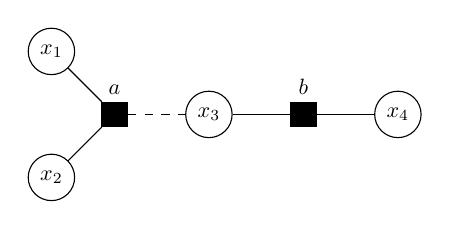
\begin{tikzpicture}[scale=0.8,transform shape]
   	\node[rectangle,draw=black, label = {$a$}, fill] (a) at (1,0) {$a$};
   	\node[rectangle,draw=black, label = {$b$}, fill] (b) at (4,0) {$a$};   
  \node[shape=circle,draw=black] (x1) at (0, 1) {$x_1$};
   
  \node[shape=circle,draw=black] (x2) at (0,-1) {$x_2$};
  \node[shape=circle,draw=black] (x3) at (2.5,0) {$x_3$};
  \node[shape=circle,draw=black] (x4) at (5.5,0) {$x_4$};
 


    
	\draw[-] (a) edge [right] node {} (x1);
	\draw[-] (a) edge [right] node {} (x2);
	\draw[-, dashed] (a) edge [right] node {} (x3);
	\draw[-] (b) edge [right] node {} (x3);
	\draw[-] (b) edge [right] node {} (x4);


\end{tikzpicture}
\end{figure}
The messages exchanged between $b$ and $x_3$ can be computed using only the definition: \newline
For example $\mu_{b \rightarrow 3}(1)$ is the probability that $(x_3 \lor x_4)$ is satisfied by an assignment where $x_3 = 1$. Its value is $1$ because each such assignment satisfy $b$. If $x_3 = 0$, only those assignments where $x_4 = 1$ will satisfy $b$ so $\mu_{b \rightarrow 3}(0) = 0.5$. \newline
Out of all 14 configurations satisfying $(x_1 \lor x_2 \lor \overline{x_3})$ there are $8$ where $x_3 = 0$ and $6$ where $x_3 = 1$, so $\mu_{3 \rightarrow b}(0) = \frac{4}{7}, \, \mu_{3 \rightarrow b}(1) = \frac{3}{7}$. 

\subsubsection{Update Rules}


\begin{wrapfigure}{r}{0.3\textwidth}

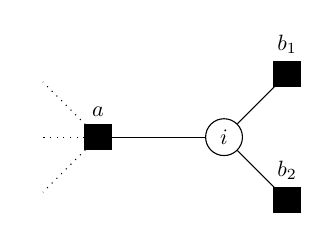
\begin{tikzpicture}[scale=0.8,transform shape]
   	\node[rectangle,draw=black, label = {$a$}, fill] (a) at (0,0) {$a$};
   	
\node[shape=circle,draw=black] (i) at (2,0) {$i$};   	
   	
   	\node[rectangle,draw=black, label = {$b_1$}, fill] (b1) at (3,1) {$a$};
   	\node[rectangle,draw=black, label = {$b_2$}, fill] (b2) at (3,-1) {$a$};

	\node[] (x1) at (-1,0) {};
	\node[] (x2) at (-1,1) {};
	\node[] (x3) at (-1,-1) {};

    \draw[dotted] (a) edge [right] node {} (x1);
    \draw[dotted] (a) edge [right] node {} (x2);
    \draw[dotted] (a) edge [right] node {} (x3);
	\draw[-] (a) edge [right] node {} (i);
	\draw[-] (i) edge [right] node {} (b1);
	\draw[-] (i) edge [right] node {} (b2);

\end{tikzpicture}
\end{wrapfigure}
$\mu_{b \rightarrow 3}(x)$, the message passed to $a$ tells the probability $i$ is $x_i = x$ considering only the factors on $i$'s side of the graph. \newline The node $i$ receives information about these factors through its neighbour vertices $b_i \neq a$. The incoming messages $\mu_{b_i \rightarrow i}(x)$ tell, if the factors are satisfied if $x_i = x$. \newline
Using Bayes theorem and the fact that $\mu_{b_i \rightarrow i}$ are conditionally independent given $x_i$, one can write the outgoing message  as a product of the incoming ones:
\begin{align*}
\mu_{i\rightarrow a}(x) = P(x_i = x \; | \; \tau_{i \rightarrow a} \text{ is sat})
&= \frac{P(x = x_i) P(x = x_i \; | \; \tau_{i \rightarrow a} \text{ is sat})}{P(\tau_{i \rightarrow a} \text{ is sat})} \\
&= \underbrace{\frac{P(x = x_i)}{P(\tau_{i \rightarrow a}\text{ is sat})}}_{C_{i \rightarrow a}} \prod_{b \neq a} \mu_{b \rightarrow i}(x) \\
\end{align*}

The factor $C_{i \rightarrow a}$ is the same for $x=0$ and $x=1$ so it suffices to compute the products for $x_i = 0$ and $x_i = 1$ and then to normalize so that $\mu_{i\rightarrow a}(0) + \mu_{i \rightarrow a}(1) = 1$. \cite{lecture} 


\begin{wrapfigure}{r}{0.3\textwidth}

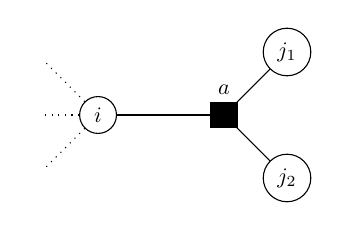
\begin{tikzpicture}[scale=0.8,transform shape]
   	\node[rectangle,draw=black, label = {$a$}, fill] (a) at (2,0) {$a$};
   	
\node[shape=circle,draw=black] (i) at (0,0) {$i$};   	
   	
   	\node[shape=circle,draw=black] (b1) at (3,1) {$j_1$};
   	\node[shape=circle,draw=black] (b2) at (3,-1) {$j_2$};

	\node[] (x1) at (-1,0) {};
	\node[] (x2) at (-1,1) {};
	\node[] (x3) at (-1,-1) {};

    \draw[dotted] (i) edge [right] node {} (x1);
    \draw[dotted] (i) edge [right] node {} (x2);
    \draw[dotted] (i) edge [right] node {} (x3);
	\draw[-] (a) edge [right] node {} (i);
	\draw[-] (a) edge [right] node {} (b1);
	\draw[-] (a) edge [right] node {} (b2);

\end{tikzpicture}
\end{wrapfigure}

To compute $\mu_{a \rightarrow i}(x_i)$ one has to sum over all configurations $X$ of the variables in $a$ where $x_i = x$. If a configuration does not satisfy $a$, it contributes nothing to $\mu_{a \rightarrow i}(x_i)$. If it does, one has to compute the probability that it also satisfies the other factors in $\tau_{a \rightarrow i}$. The probability that a configuration where $j$ takes the value $x_j$ satisfies the factors behind the neighbour variable $j$ is $\mu_{j \rightarrow a}(x_j)$. Again these probabilities are independent and the probability for all factors is simply the product.

$$\mu_{a \rightarrow i}(x) = \sum_{ X = \{x_j (j \neq i), \; x_i = x\}} f_a(X) \prod_{j \neq i} \mu_{j \rightarrow a}(x_j)$$


\begin{example}
Now the messages from the first example can be computed with belief propagation.
% $$\mathcal{F} = \underbrace{(x_1 \lor x_2 \lor \overline{x_3})}_a  \land \underbrace{(x_3 \lor x_4)}_b $$
Since the formula's factor graph is a tree, the updates can be scheduled so that each message has to be computed only once.

\begin{itemize}
\item Level 0 (Leaves)

The leaves are all variable nodes. As they receive no incoming messages they will all send the same constant message. The empty product in the update rule evaluates to $1$, after normalization the values are \newline $\mu_{1 \rightarrow a}(0) = \mu_{1 \rightarrow a}(1) = 1/2$. The same holds for $2 \rightarrow a$ and $4 \rightarrow b$.

\item Level 1
The message of level $1$ are both sent from factors to variables: 
\begin{align*}
\mu_{a \rightarrow 3}(0) = &\mu_{1 \rightarrow a}(0)\mu_{2 \rightarrow a}(0) + \mu_{1 \rightarrow a}(0)\mu_{2 \rightarrow a}(1) + \mu_{1 \rightarrow a}(1) \mu_{2 \rightarrow a}(0) \\ + & \mu_{1 \rightarrow a}(1)\mu_{2 \rightarrow a}(1) = 1 \\
\mu_{a \rightarrow 3}(1) = &\mu_{1 \rightarrow a}(0)\mu_{2 \rightarrow a}(1) + \mu_{1 \rightarrow a}(1) \mu_{2 \rightarrow a}(0) + \mu_{1 \rightarrow a}(1)\mu_{2 \rightarrow a}(1) \\ = &3/4 \\
\mu_{b \rightarrow 3}(0) = &\mu_{4 \rightarrow b}(1) = 1/2 \\
\mu_{b \rightarrow 3}(1) = &\mu_{4 \rightarrow b}(0) + \mu_{4 \rightarrow b}(1) = 1
\end{align*}

\item Level 2
The unnormalized values for $3 \rightarrow b$ are $0.5$ and $1$. After normalization one gets $\mu_{3 \rightarrow b}(0) = \frac{0.5}{0.5 + 1} = \frac{1}{3}$ and $\mu_{3 \rightarrow b}(1) = \frac{2}{3}$. \newline
The values $\mu_{3 \rightarrow a}(0) = \frac{1}{1 + 0.75} = \frac{4}{7}$ and $\mu_{4 \rightarrow a}(1) = \frac{3}{7}$ are obtained in the same way.
%  \item Level 3

\end{itemize}
The values for the remaining 3 edges of level $4$ can be looked up in the tabular

\end{example}

\begin{figure}[h]
\begin{floatrow}
\centerfloat
\capbtabbox{%
  \begin{tabular}{ccc} \hline
  Edge & $\mu(0)$ & $\mu(1)$ \\ \hline
  $1 \rightarrow a$ & $1/2$ & $1/2$ \\
  $2 \rightarrow a$ & $1/2$ & $1/2$ \\ 
  $4 \rightarrow b$ & $1/2$ & $1/2$ \\ 
  $a \rightarrow 3$ & $1$   & $3/4$ \\ 
  $b \rightarrow 3$ & $0.5$ & $1$ \\ 
  $3 \rightarrow a$ & $1/3$ & $2/3$ \\ 
  $3 \rightarrow b$ & $3/7$ & $4/7$ \\ 
  $a \rightarrow 2$ & $5/6$ & $1$ \\ 
  $a \rightarrow 2$ & $1$ & $5/6$ \\ 
  $b \rightarrow 1$ & $4/7$ & $1$ \\ 
  \end{tabular}
}{}
%{%
%  \caption{A table}%
%}
\ffigbox{%
  \centering
  \centerfloat
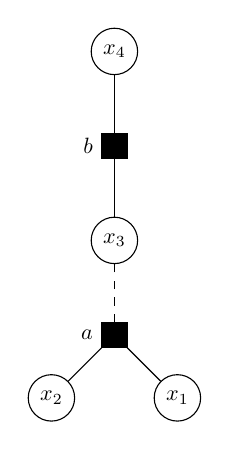
\begin{tikzpicture}[scale=0.8,transform shape]
   	\node[rectangle,draw=black, label = left:{$a$}, fill] (a) at (0,1) {$a$};
   	\node[rectangle,draw=black, label = left:{$b$}, fill] (b) at (0,4) {$a$};   
  \node[shape=circle,draw=black] (x1) at (1, 0) {$x_1$};
   
  \node[shape=circle,draw=black] (x2) at (-1,0) {$x_2$};
  \node[shape=circle,draw=black] (x3) at (0,2.5) {$x_3$};
  \node[shape=circle,draw=black] (x4) at (0,5.5) {$x_4$};
 


    
	\draw[-] (a) edge [right] node {} (x1);
	\draw[-] (a) edge [right] node {} (x2);
	\draw[-, dashed] (a) edge [right] node {} (x3);
	\draw[-] (b) edge [right] node {} (x3);
	\draw[-] (b) edge [right] node {} (x4);


\end{tikzpicture}


}{%
  %\caption{A figure}%
}
\end{floatrow}
\end{figure}



In \cite{survprob} the standard BP rules are expressed in a different, but equivalent way: \newline
Instead of computing $\mu_{i \rightarrow a}(0)$ and $\mu_{i \rightarrow a}(1)$ which add up to $1$, one can also compute the value $\gamma_{i \rightarrow a}$, the probability that $x_i$ violates $a$. 
It can be expressed as $\gamma_{i \rightarrow a} = \left\{
  \begin{array}{@{}ll@{}}
    \mu_{i \rightarrow a}(0) & \text{if}\ J_a^i = 1 \\
    \mu_{i \rightarrow a}(1), &  \text{if}\ J_a^i = 0
  \end{array}\right\}$
  
The message sent from $a$ to $i$ is the probability that all neighbour variables $j \neq i$ would violate $a$: $\delta_{a \rightarrow i} = \prod_{j \neq i} \gamma_{j \rightarrow a}$ which is already the first update equation for the modified BP version.
The opposite direction $i \rightarrow a$ is the more complicated one: 
Like in the WP-update the variable $i$ may satisfy $a$, if for \emph{none} of its other neighbours $b$ with $J_b^i \neq J_a^i$ fixes $i$. In terms of BP messages the probability for this situation is $$P_{i \rightarrow a}^s = \prod_{b \in V_a^u(i)}(1 - \delta_{b \rightarrow i})$$
The same applies to the probability that $i$ may violate $a$: 
 $$P_{i \rightarrow a}^u = \prod_{b \in V_a^s(i)}(1 - \delta_{b \rightarrow i})$$

The values $P_{i \rightarrow a}^u$ and $P_{i \rightarrow a}^s$ are exactly 

Like in the original update for $\mu_{i \rightarrow a}$ the value of \
\subsection{Marginal Probabilities}

\subsection{Number of satisfying assignments}